% !TeX root = ../../../main.tex
\begin{figure}[htbp]
\begin{ChFiveFloatBody}

\centering

\begin{minipage}[t]{0.49\linewidth}
    \centering
    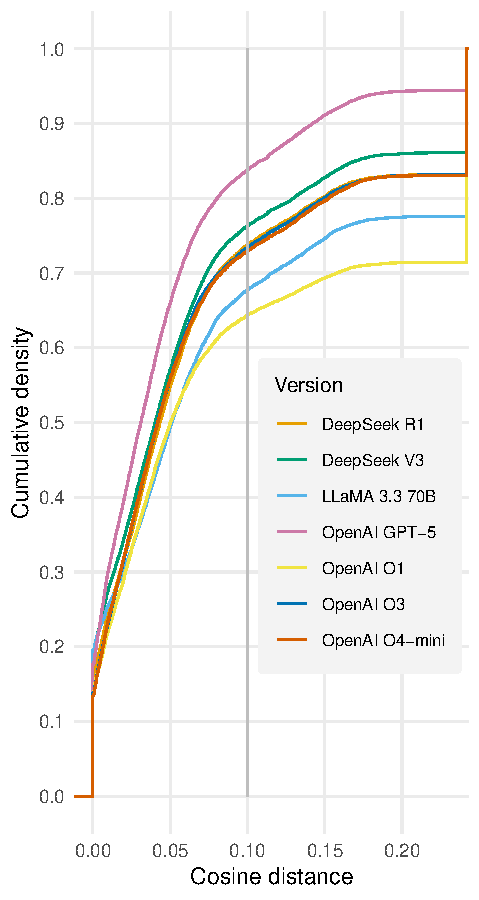
\includegraphics[
        page=1,
        width=0.8\linewidth
    ]{Chapters/chapter-05/images/Plots_tables/pmoa_updated_man_figs.pdf}
\end{minipage}
\hfill
\begin{minipage}[t]{0.49\linewidth}
    \centering
    \includegraphics[
        page=2,
        width=0.8\linewidth
    ]{Chapters/chapter-05/images/Plots_tables/pmoa_updated_man_figs.pdf}
\end{minipage}

\par\medskip

\begin{minipage}[t]{0.49\linewidth}
    \centering
    \includegraphics[
        page=3,
        width=0.8\linewidth
    ]{Chapters/chapter-05/images/Plots_tables/pmoa_updated_man_figs.pdf}
\end{minipage}
\hfill
\begin{minipage}[t]{0.49\linewidth}
    \centering
    \includegraphics[
        page=4,
        width=0.8\linewidth
    ]{Chapters/chapter-05/images/Plots_tables/pmoa_updated_man_figs.pdf}
\end{minipage}





\end{ChFiveFloatBody}
\caption{
Comparison of different LLMs for extracting temporal clinical events
from case reports:
(\textbf{A}) cumulative distribution of event-matching cosine distances;
(\textbf{B}) temporal-concordance box plots;
(\textbf{C}) timestamp discrepancies between model-generated and manual
annotations among semantically matched events; and
(\textbf{D}) timestamp discrepancies stratified by the clinician-annotated
time relative to presentation.
}\ChFiveFloatLabel{ch05:fig:tts_evaluation}
\end{figure}